\section{Tecnologie utilizzate}

Dal punto di vista delle piattaforme, degli strumenti operativi e delle pratiche di deployment, l’ambiente tecnologico osservato durante lo stage combina soluzioni \emph{enterprise} 
consolidate con strumenti e approcci moderni orientati alla scalabilità, all’integrazione e all’automazione. 
Di seguito viene fornita una descrizione estesa delle tecnologie principali e del loro impatto operativo.

\medskip
\noindent\textbf{Salesforce Commerce Cloud}
\emph{Salesforce Commerce Cloud} e relativi moduli \emph{Service Cloud} / \emph{Marketing Cloud} (suite \emph{enterprise} per commercio, servizio clienti e automazione marketing): 
queste piattaforme vengono impiegate per realizzare soluzioni di commercio elettronico e gestione clienti sia in ambito \emph{B2B} che \emph{B2C}. Nell’uso osservato, la suite supporta 
integrazioni con sistemi esterni per sincronizzare cataloghi, ordini e dati anagrafici; consente la personalizzazione della \emph{customer experience} tramite regole di business e strumenti di segmentazione,
e automatizza attività di marketing e customer care. Dal punto di vista operativo richiede competenze specifiche per la gestione delle estensioni, delle API e dei processi di deployment 
verso ambienti proprietari della piattaforma.

\begin{figure}[htbp]
    \centering
    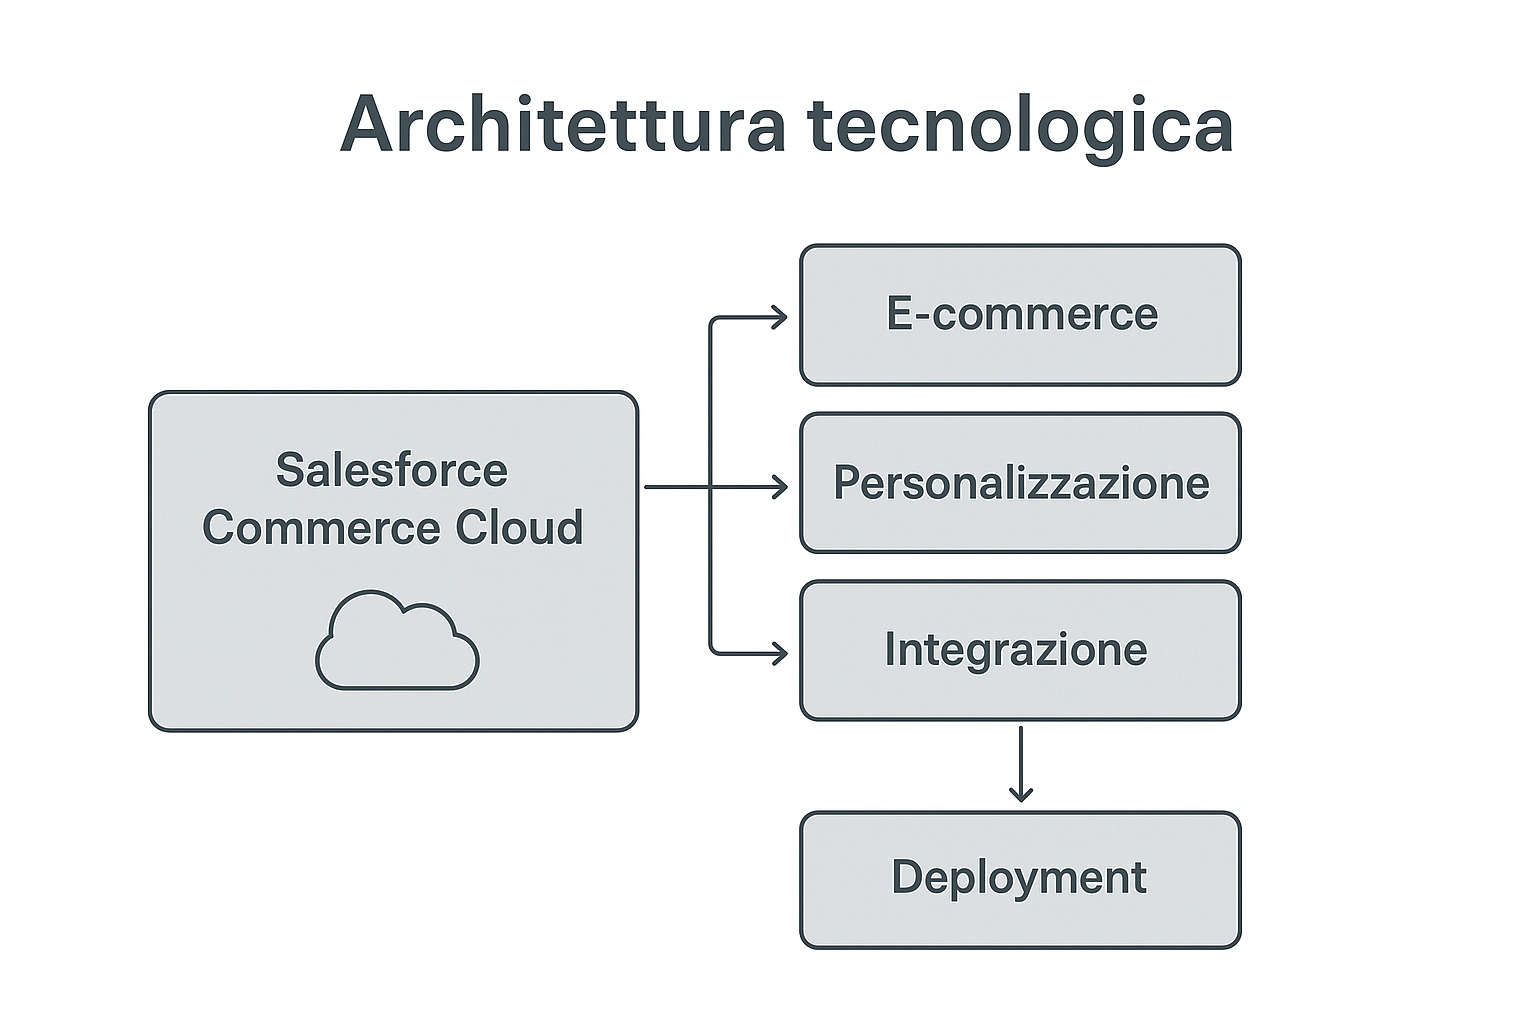
\includegraphics[width=0.9\textwidth]{images/azienda/architettura_tecnologica.svg}
    \caption{Architettura tecnologica osservata: le principali piattaforme e i flussi di integrazione tra e-commerce, personalizzazione, integrazione e deployment.}
    \label{fig:architettura_tecnologica}
\end{figure}


\medskip
\noindent\textbf{Bloomreach}
\emph{Bloomreach} (piattaforma per ricerca avanzata e personalizzazione della \emph{customer journey}): utilizzata in progetti di scala per migliorare la rilevanza delle ricerche 
interne al sito e per orchestrare contenuti personalizzati lungo il percorso di acquisto. Bloomreach funge da livello di personalizzazione e ricerca ad alto throughput, spesso integrato 
con il \emph{CMS} e il \emph{CRM} per arricchire i profili utente e abilitare esperienze omnicanale.

\medskip
\noindent\textbf{deployment}
Cloud e piattaforme di \emph{deployment}: \emph{AWS}, \emph{Google Cloud} e \emph{Heroku} per hosting, provisioning di risorse scalabili e ambienti di \emph{staging} e \emph{production}. 
Queste piattaforme vengono impiegate per ospitare servizi applicativi, database e risorse di caching; la scelta tra le piattaforme è dettata da vincoli di progetto, integrazioni richieste e costi operativi. 
Sul cloud si realizzano inoltre configurazioni per il \emph{scaling} automatico, il bilanciamento del carico e la gestione dei certificati TLS. Per l’infrastruttura 
è comune l’adozione di pratiche di \emph{infrastructure as code} (ad es. strumenti che consentono il provisioning ripetibile delle risorse).

\begin{figure}[htbp]
    \centering
    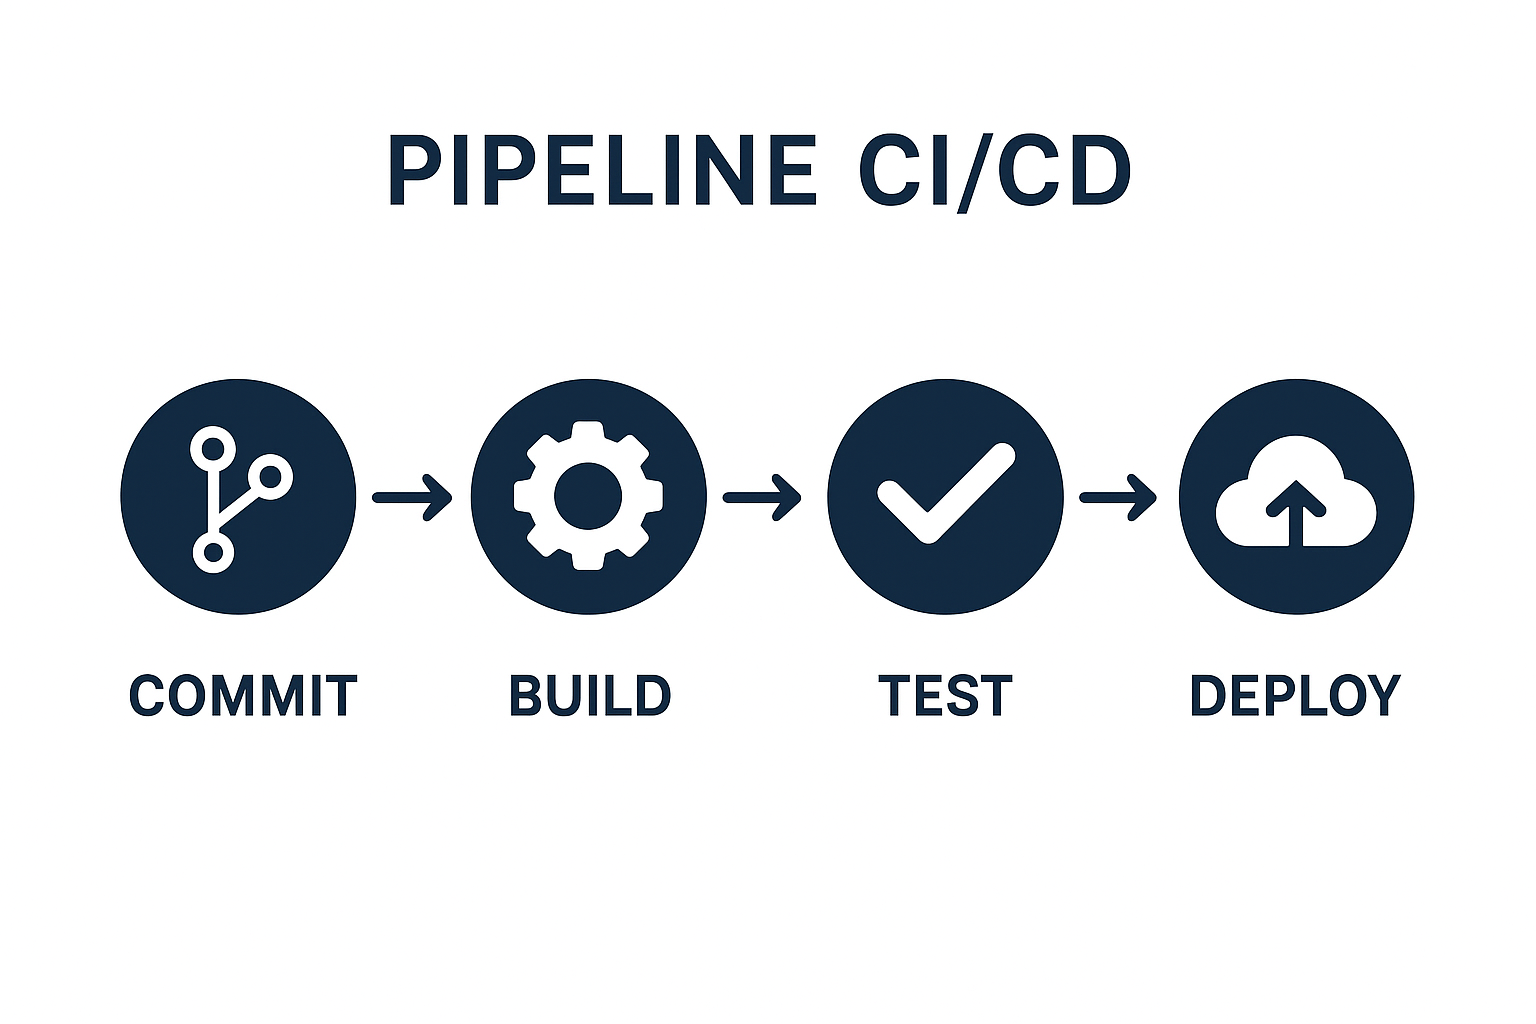
\includegraphics[width=0.85\textwidth]{images/azienda/pipeline_cicd.svg}
    \caption{Pipeline di integrazione e distribuzione continua: dal commit alla promozione in produzione.}
    \label{fig:pipeline_cicd}
\end{figure}

% [Develop] → [Commit su Git] → [CI Build] → [Test automatici] → [Code review / Pull Request] → [Merge su main] → [Deploy su Staging] → [Verifica] → [Deploy in Production]


\medskip
\noindent\textbf{iPaaS}
Strumenti di integrazione: approcci punto a punto e soluzioni \emph{iPaaS} (\emph{Integration Platform as a Service}: piattaforme per orchestrare integrazioni) 
per orchestrare flussi dati fra \emph{CRM}, \emph{ERP}, piattaforme e-commerce e \emph{CMS}. L’impiego di un \emph{iPaaS} semplifica la gestione degli \emph{endpoint}, 
la trasformazione dei payload e la gestione degli errori/ritentativi, riducendo la complessità rispetto a molteplici integrazioni punto-a-punto. Nei progetti osservati, 
le integrazioni includono sincronizzazione ordini, anagrafiche clienti, disponibilità di magazzino e tracking degli eventi di marketing.

\medskip
\noindent\textbf{Gestione progetto}
Strumenti di gestione progetto e comunicazione: \emph{Jira} per il tracciamento delle attività e \emph{Slack} per la comunicazione operativa quotidiana. \emph{Jira} 
viene usato per definire le \emph{issue}, assegnare priorità, documentare criteri di accettazione e tenere traccia dello stato di avanzamento; \emph{Slack} 
è lo strumento preferito per aggiornamenti rapidi, notifiche dagli strumenti di integrazione (build, deploy, alert) e conversazioni sincrone o asincrone tra membri del \emph{team}.

\medskip
\noindent\textbf{Git}
Controllo versione e \emph{pipeline}: uso diffuso di \emph{Git}, \emph{pipeline} di integrazione continua (\emph{CI}) e distribuzione continua (\emph{CD}) e \emph{test} 
automatici (ad esempio \emph{unit tests} e \emph{integration tests}) prima del rilascio. Il flusso di lavoro tipico prevede sviluppo su \emph{feature branches}, 
apertura di \emph{pull request} per la revisione del codice (\emph{code review}), esecuzione automatica di test nella \emph{pipeline} e successiva promozione verso 
ambienti di \emph{staging} e infine \emph{production}. Strategie di rilascio come \emph{blue/green} o \emph{canary} possono essere adottate per minimizzare il 
rischio in produzione, così come meccanismi di rollback automatizzato in caso di regressione.

A livello operativo queste tecnologie si traducono in pratiche concrete (osservate però solo in parte durante lo stage) che includono:

\begin{itemize}
\item sviluppo su rami funzionali con revisioni del codice (\emph{code review}) formali e commenti tracciati tramite \emph{pull request} o meccanismi equivalenti;
\item creazione e gestione di ambienti distinti di \emph{staging} e \emph{production} sul cloud, con pipeline che automatizzano build, test e deployment;
\item esecuzione di \emph{test} automatici a livelli differenziati (\emph{unit}, \emph{integration}, \emph{end-to-end}) per garantire qualità e ridurre regressioni;
\item strumenti di monitoraggio e \emph{logging} centralizzati per osservabilità e diagnosi (alerting su metriche critiche, raccolta dei log applicativi e centralizzazione dei tracciati di errore);
\item pratiche di sicurezza e compliance applicate alle integrazioni e al trattamento dei dati (gestione di credenziali, accessi basati su ruoli, cifratura dei dati sensibili in transito e a riposo).
\end{itemize}

\medskip

\noindent\textbf{Implicazioni operative e suggerimenti}

L’adozione di questo insieme di tecnologie determina alcuni vincoli e opportunità operative: la complessità delle integrazioni richiede governance dei \emph{data contracts} e 
politiche chiare di versioning delle API; le piattaforme \emph{enterprise} come \emph{Salesforce Commerce Cloud} richiedono competenze specifiche per personalizzazioni e upgrade; 
le risorse cloud implicano attenzione alla gestione dei costi e al monitoraggio del consumo. Per migliorare l’efficacia complessiva è raccomandabile formalizzare convenzioni comuni 
(naming delle \emph{branches}, standard per le \emph{code review}, soglie di qualità per le \emph{pipeline}) e prevedere un minimo di documentazione operativa a supporto dell’onboarding e della manutenzione.

In conclusione, la suite tecnologica osservata mette a disposizione strumenti potenti per costruire soluzioni integrate e scalabili; la sfida principale risiede nell’armonizzare pratiche, 
automazioni e governance per trasformare la tecnologia in valore ripetibile e manutenibile nel tempo.


%Per la manutenzione e il supporto operativo si privilegia un approccio a livelli: monitoraggio dei servizi e dei log, 
%gestione dei \emph{ticket} tramite \emph{Jira} e interventi pianificati per aggiornamenti e patch. Nei progetti di maggiori 
%dimensioni si osserva una separazione tra team di sviluppo (feature delivery) e team di \emph{platform/operations} (monitoraggio, sicurezza, scaling), 
%mentre per clienti più piccoli le stesse persone spesso ricoprono più ruoli.

%Infine, la scelta delle tecnologie è stata chiaramente guidata dalla dimensione e dalla strategia del cliente: soluzioni \emph{Shopify} per rollout rapidi e basso \emph{TCO} 
%(\emph{Total Cost of Ownership}: costo totale di proprietà); architetture \emph{headless} e piattaforme \emph{Salesforce} per scenari enterprise e integrazioni complesse. 
%Ho inoltre riscontrato una forte propensione dell’azienda verso l’adozione di tecnologie emergenti legate all'\emph{AI} e alla personalizzazione, 
%inserite come componenti modulari (ad esempio agenti intelligenti collegati al \emph{CRM} o servizi di personalizzazione integrati con \emph{Bloomreach}). 
%In sintesi, l’ambiente tecnologico è eterogeneo e modulare, concepito per supportare sia progetti a rapido lancio sia soluzioni enterprise complesse, 
%con attenzione all’innovazione e alla scalabilità operativa.
%Sezione in cui verrà descritto il contesto produttivo in cui sono stato inserito, con particolare attenzione alle tecnologie operative viste adottare.
